\section{Introdução}
%%%%%%%%%%%%%%%%%%%%%%%%%%%%%%%%%%%%%%%%%%%%%%%%%%%%%%%%%%%%%%%%
\begin{frame}
\frametitle{\textcolor{green}{Sensor}}
Célula de Peso.
\begin{figure}[!b]
	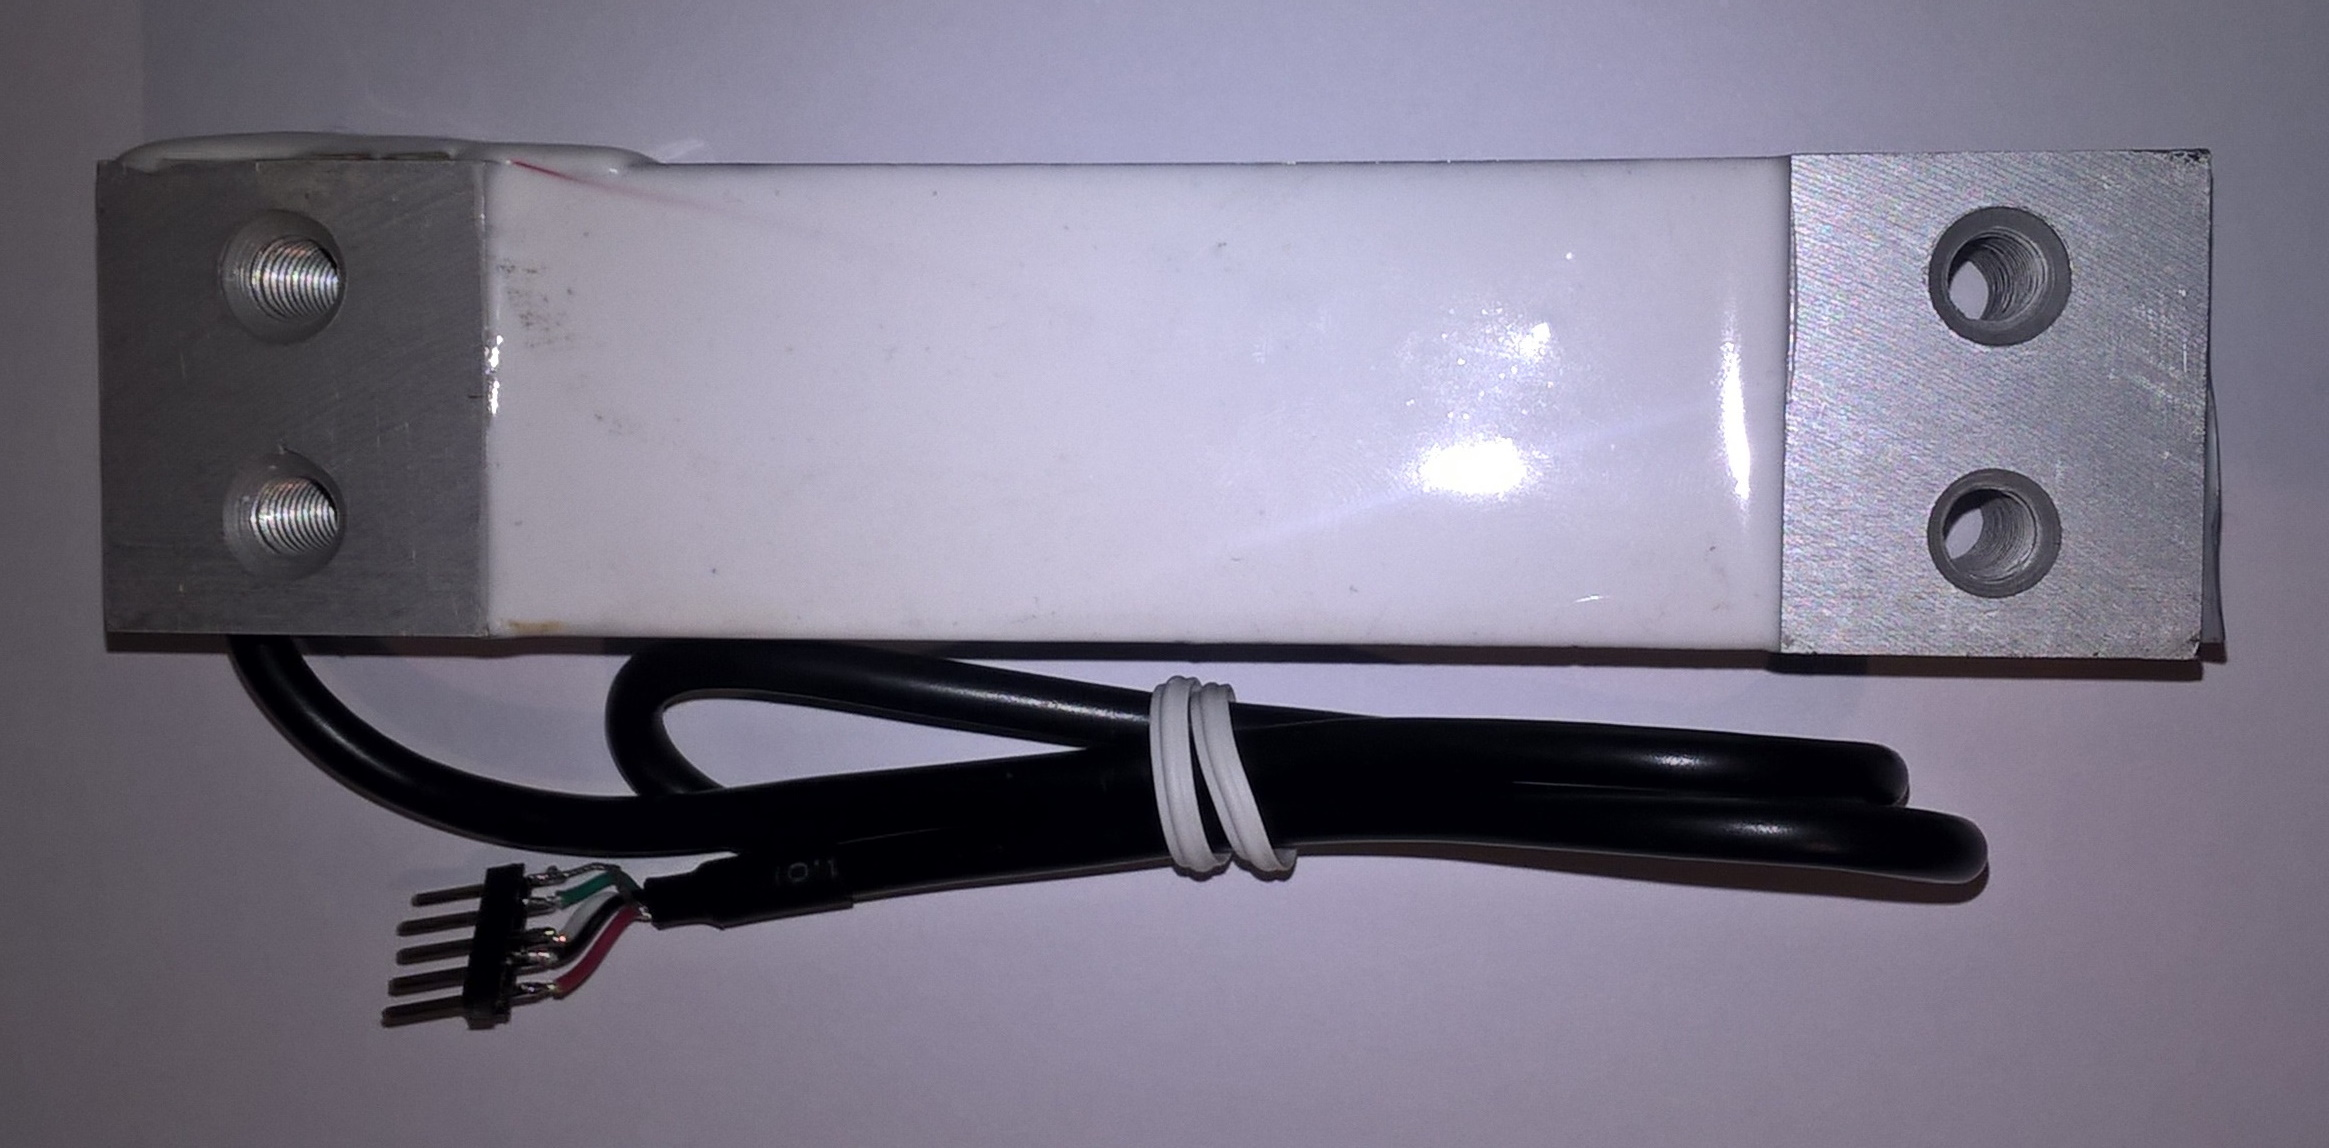
\includegraphics[scale=0.08]{./image/PESTA/material/Load_Cell_1.jpg}
	\hspace{.1cm}
	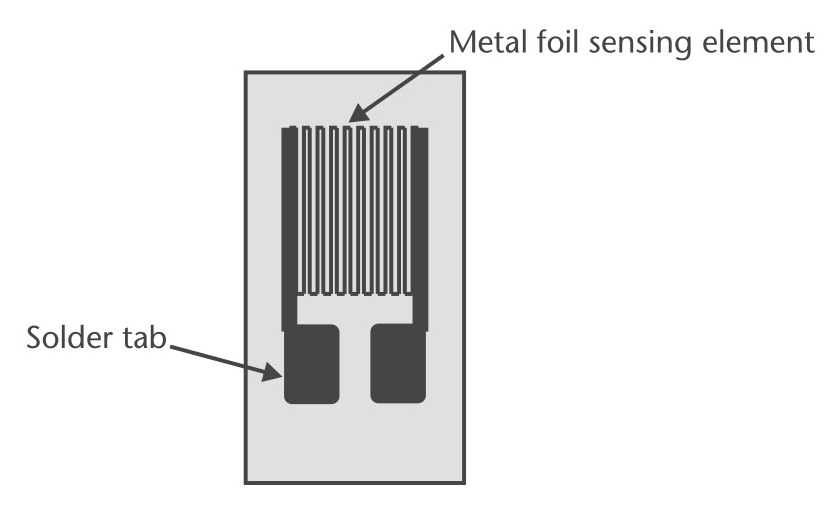
\includegraphics[scale=.1]{./image/PESTA/general/strain_gauge_1.jpg}
	\hspace{.1cm}
	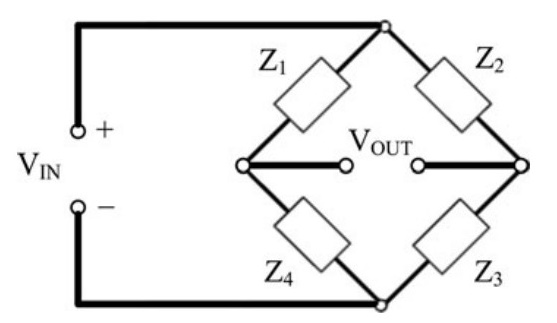
\includegraphics[scale=.3]{./image/PESTA/schematic/Wheatstone_Bridge_1.jpg}
\end{figure}
Sensores piezoresistivos ligados na forma de ponte de \textit{Wheatstone}.
\newline
\newline
O efeito foi descoberto pela primeira vez por Lord Kelvin em \textcolor{blue}{1856}, e a primeira aplicação do efeito piezoresistivo não apareceu até a década de \textcolor{blue}{1930}, cerca de \textcolor{blue}{75} anos após sua descoberta.
\end{frame}
%%%%%%%%%%%%%%%%%%%%%%%%%%%%%%%%%%%%%%%%%%%%%%%%%%%%%%%%%%%%%%%%
\begin{frame}
\frametitle{\textcolor{green}{Amplificador}}
\textit{Load Cell Amplifier} [HX711]
\begin{figure}[H]
	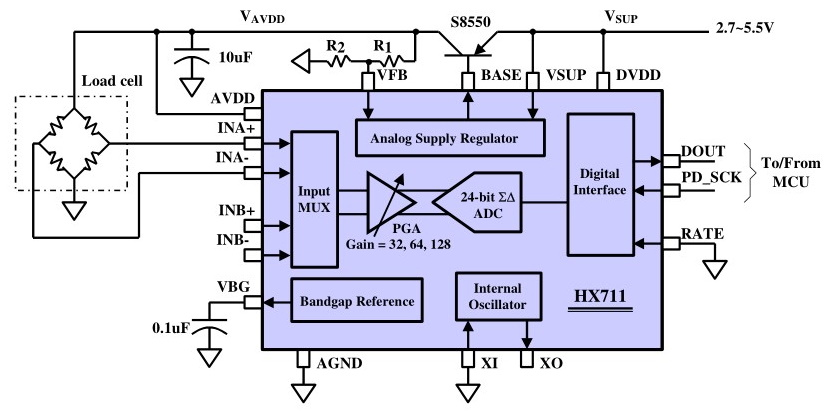
\includegraphics[scale=0.25]{./image/PESTA/schematic/HX711_Schematic_1.jpg}
	\hspace{2cm}
	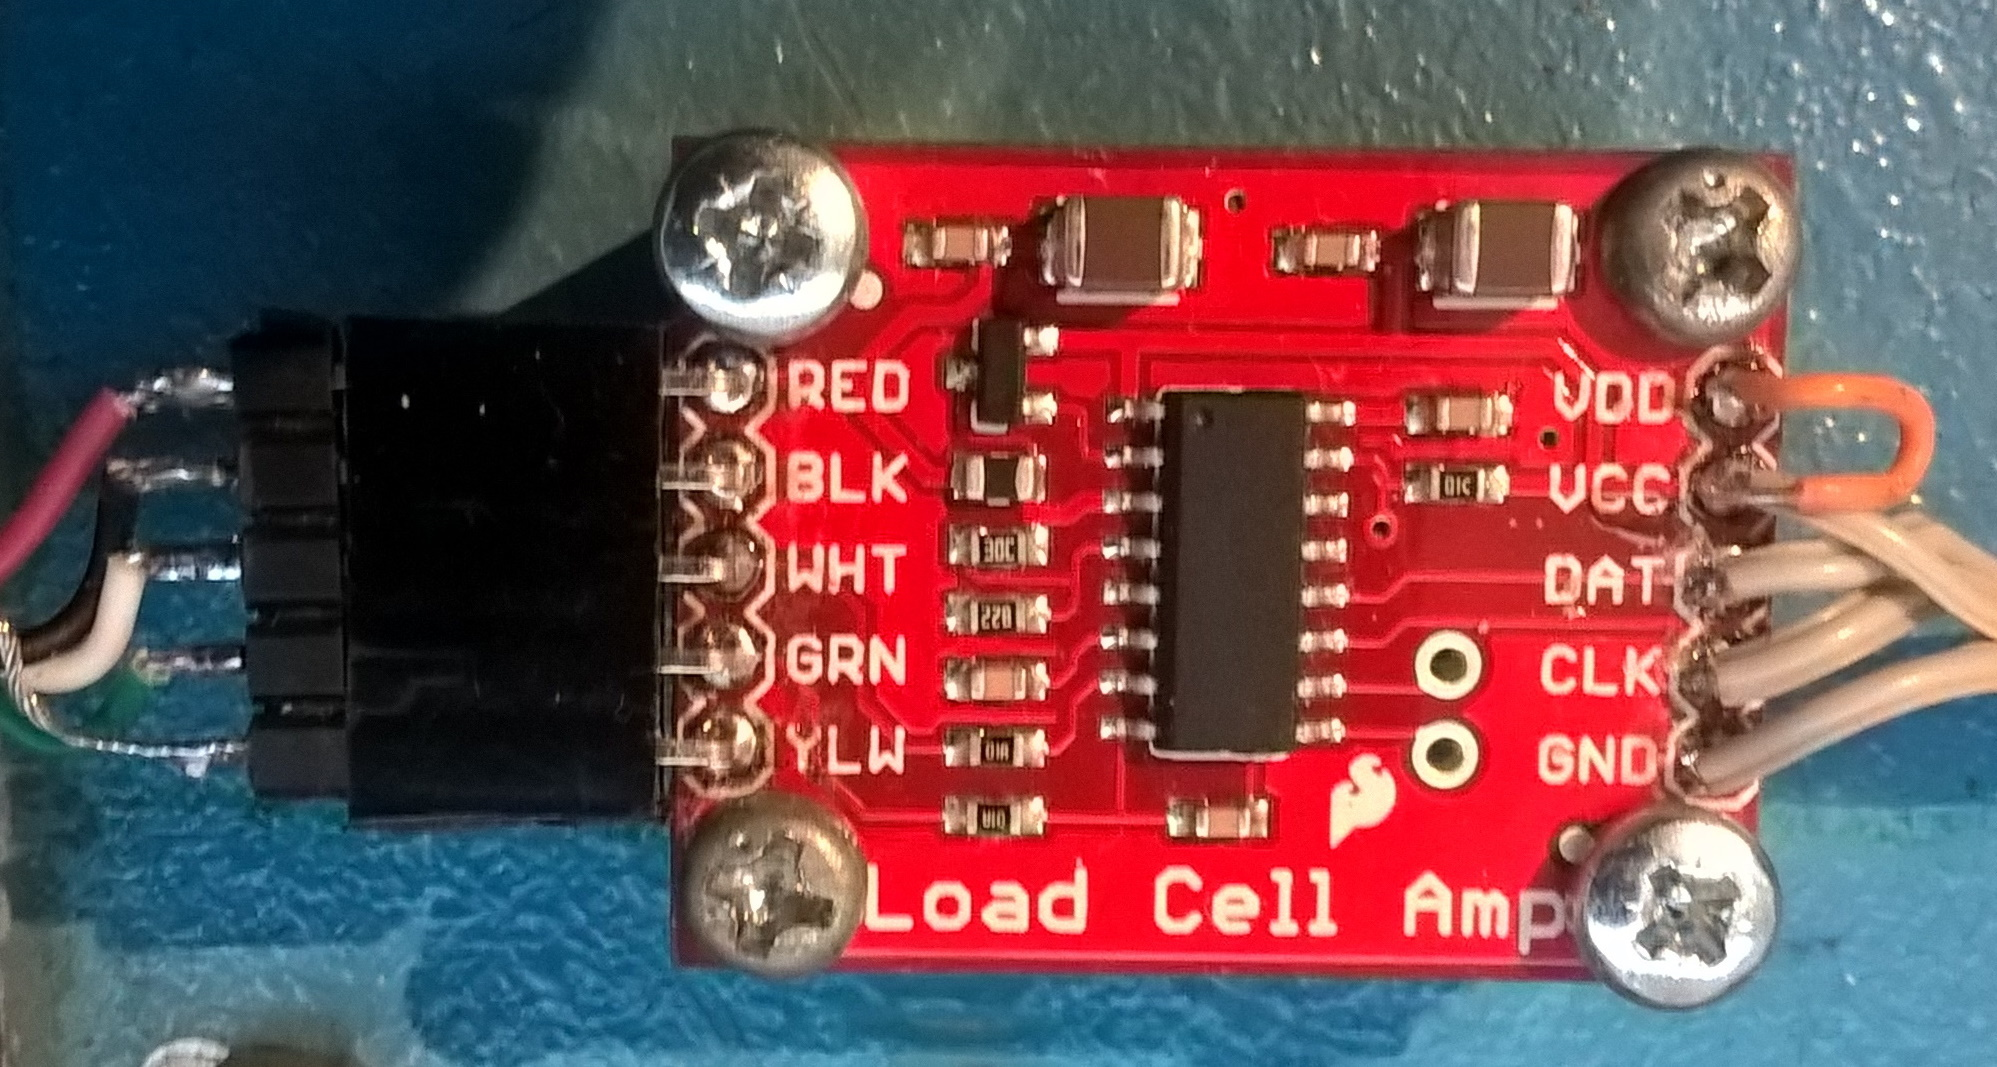
\includegraphics[scale=0.05]{./image/PESTA/material/HX711_board_1.jpg}
\end{figure}
\begin{itemize}
	\item \textcolor{blue}{10} ou \textcolor{blue}{80} amostras por segundo.
	\item Protocolo de comunicação proprietário.
	\item Filtro de ruido da rede \textcolor{blue}{50}, \textcolor{blue}{60} Hz.
	\item Dois canais com ganhos programáveis por software.
	\item \textcolor{blue}{24} \textit{bit} de resolução, etc
\end{itemize}
\end{frame}
%%%%%%%%%%%%%%%%%%%%%%%%%%%%%%%%%%%%%%%%%%%%%%%%%%%%%%%%%%%%%%%%

